\myChapter{Experiments}
\label{chap:Experiments}

In this chapter, we will showcase various experiments and their corresponding results, highlighting the inference speed and image quality. We will utilize both the basic PyTorch implementations of UNET and SRUNET, as well as their compiled counterparts with TensorRT, which will be configured with different precisions for weights/activations, namely FP32, FP16, and INT8.

Most interesing facts:
\begin{itemize}
\item{
  From \cref{tab:tab1}, INT8 models outperform full-precision performance on non-perceptual metrics, such as SSIM, PSNR, MS-SSIM. This is probably due to the fact that outputs from lower precision models are naturally more blurry than the ones from full-precision models.
}

\item{
  Images generated by plain PyTorch implementations and their FP32 versions differ in quality most likely because they differ at the end of their architectures, since they use respectively bicubic and bilinear interpolation techniques to scale up the input low-quality image to allow the models to learn residual values between low- and high-quality images.
}

\end{itemize}
\section{Quantitative Results}

\Cref{tab:tab1} shows the average value of each IQA metric for each model variation, along with the standard deviation (shown as ±). The values in the table indicate the quality of the images generated by the models, with higher values indicating better quality.
LPIPS and BRISQUE metrics underline strong differences between plain PyTorch implementations and their relative TRT ones for both UNET and SRUNET, the same can be said of PSNR, while SSIM and MS\_SSIM stay in the same range of values for each model variation.

\Cref{tab:tab2} shows the execution times (in seconds) of different variations of UNET and SRUNET implementations. Each table entry represents the average execution time over more than 300 executions "±" its standard deviation. SRUNET generally has faster execution times than UNET across all numerical precisions. Among the different numerical precisions, the fastest execution times are generally achieved, as expected by using INT8, followed by FP16 and FP32.

TODO: increase precision of times table

TODO: decrease precision of metrics table and add VMAF

\begin{table*}[t]
\begin{tabular}{llllll}
\toprule
{} &          LPIPS &           SSIM &            PSNR &        MS\_SSIM &         BRISQUE \\
\midrule
UNET        &  0.559 ± 0.007 &  0.879 ± 0.004 &  21.939 ± 0.027 &  0.735 ± 0.002 &   153.591 ± 0.0 \\
UNET\_FP32   &  0.354 ± 0.011 &  0.897 ± 0.003 &   28.64 ± 0.108 &  0.871 ± 0.003 &   26.783 ± 1.83 \\
UNET\_FP16   &  0.354 ± 0.011 &  0.897 ± 0.003 &   28.64 ± 0.108 &  0.871 ± 0.003 &   26.788 ± 1.84 \\
UNET\_INT8   &  0.343 ± 0.011 &  0.895 ± 0.003 &  28.613 ± 0.108 &   0.87 ± 0.003 &  26.448 ± 1.694 \\
SRUNet      &  0.551 ± 0.008 &  0.869 ± 0.004 &  19.303 ± 0.014 &  0.669 ± 0.002 &   153.591 ± 0.0 \\
SRUNet\_FP32 &  0.396 ± 0.012 &  0.896 ± 0.003 &  28.837 ± 0.126 &  0.871 ± 0.003 &  34.647 ± 2.336 \\
SRUNet\_FP16 &  0.396 ± 0.012 &  0.896 ± 0.003 &  28.837 ± 0.126 &  0.871 ± 0.003 &  34.642 ± 2.334 \\
SRUNet\_INT8 &  0.373 ± 0.012 &  0.895 ± 0.003 &  28.806 ± 0.124 &  0.869 ± 0.003 &  34.868 ± 1.989 \\
\bottomrule
\end{tabular}
\caption{Evaluation metrics over 50 frames (mean $\pm$ standard deviation).}
\label{tab:tab1}
\end{table*}

\begin{table*}[t]
\begin{tabular}{ll}
\toprule
{} &      times [s] \\
\midrule
UNET        &    0.035 ± 0.0 \\
UNET\_FP32   &  0.028 ± 0.001 \\
UNET\_FP16   &  0.028 ± 0.001 \\
UNET\_INT8   &    0.015 ± 0.0 \\
SRUNet      &    0.012 ± 0.0 \\
SRUNet\_FP32 &  0.009 ± 0.001 \\
SRUNet\_FP16 &    0.009 ± 0.0 \\
SRUNet\_INT8 &    0.006 ± 0.0 \\
\bottomrule
\end{tabular}
\caption{Evaluation times over 1000 runs (mean $\pm$ standard deviation).}
\label{tab:tab2}
\end{table*}

\section{Qualitative Results}

TODO: make figure captions shorter and describe such images.

TODO: adjust figures positioning

\begin{figure*}[h]
  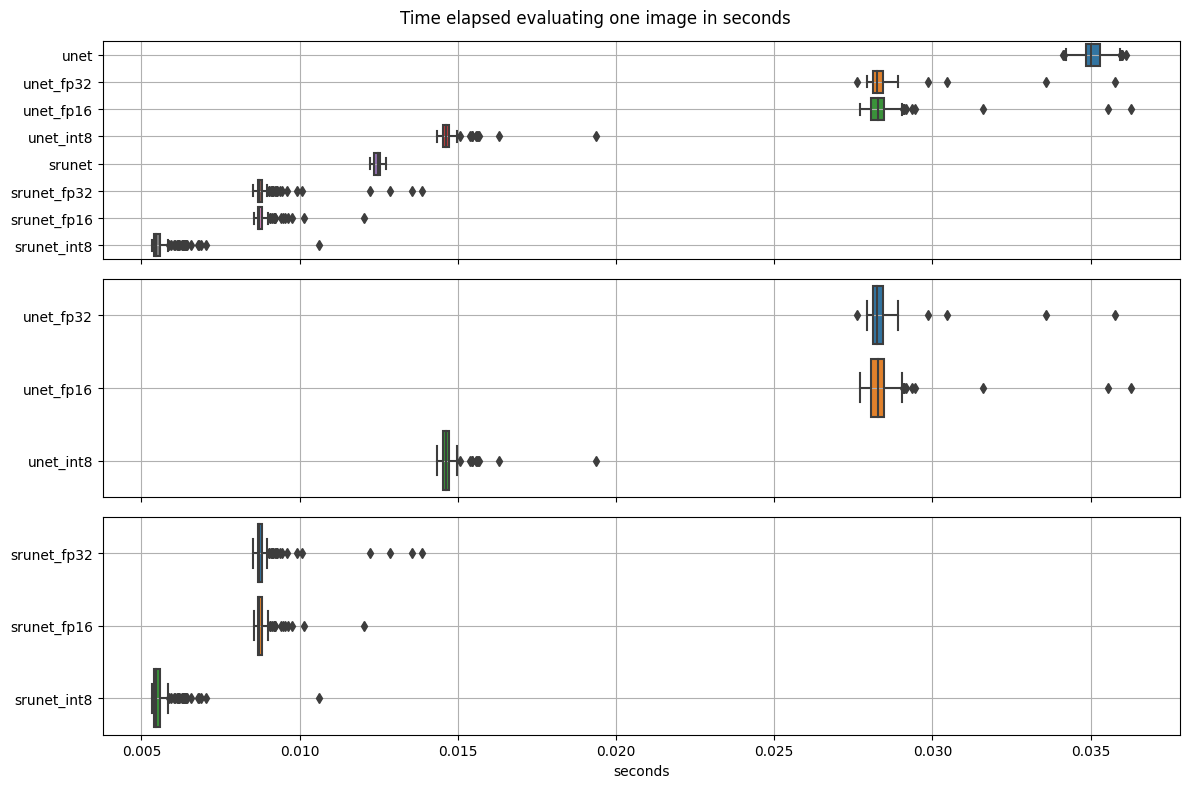
\includegraphics[width=1.0\textwidth]{static/2023_03_02_boxplots_timings_all.png}
  \caption{Average times elapsed in seconds for generating one image using different versions of UNET and SRUNET implementations. The top graph shows all the versions, the middle one zooms in comparing only the TRT versions of UNET, as well as the bottom graph for SRUNET.}
\end{figure*}

\begin{figure*}[h]
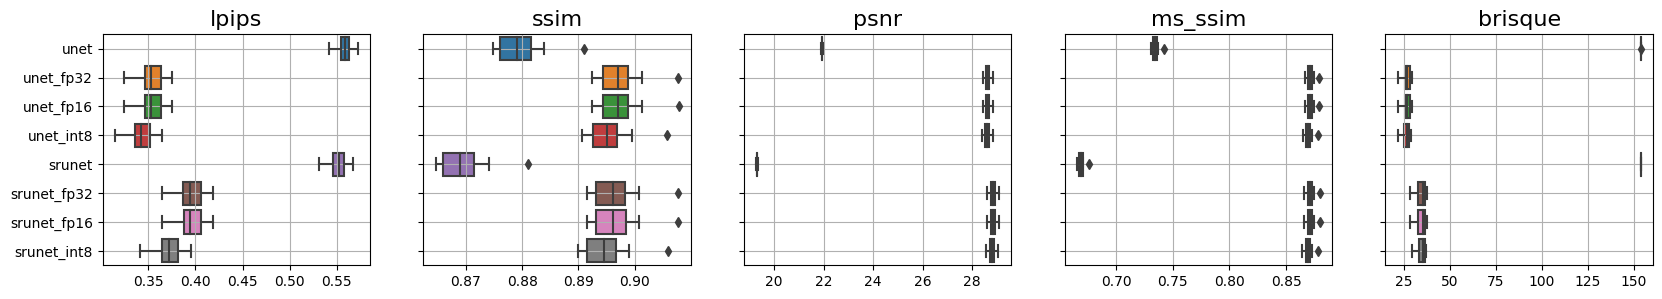
\includegraphics[width=1.0\textwidth]{static/2023_03_02_boxplots_metrics_all.png}
\caption{Average results for some IQA metrics on validation images with different versions of UNET and SRUNET implementations.}
\end{figure*}

\begin{figure*}[h]
\includegraphics[width=1.0\textwidth]{static/2023_03_02_boxplots_metrics_quant_SRUNet.png}
\caption{Average results for some IQA metrics on validation images with different versions of UNET implementations.}
\end{figure*}

\begin{figure*}[h]
\includegraphics[width=1.0\textwidth]{static/2023_03_02_boxplots_metrics_quant_UNET.png}
\caption{Average results for some IQA metrics on validation images with different versions of SRUNet implementations.}
\end{figure*}

\pagebreak


